\chapter{Conclusion}\label{chap:Conclusion} \markright {\thechapter~Conclusion}

\section{Sustainability assessment criteria}
The GWP and construction cost are treated as primary assessment criteria for sustainability to respect the ecological and the economical dimensions.

It was observed, that for concrete systems, ecological better performing systems also became economically valid. Showing that initial complexity for concrete structures does pay-off generally for spans above $7m$.

Construction height is also identified as a primary criterion, as it can directly affect the number of possible storeys within a fixed building envelope and therefore influence the usable floor area. 

Mass is considered a secondary criterion for residential buildings, since acoustic floor build-ups reduce the differences in total system weight. For office buildings, mass is more relevant because the total weight is governed more directly by the structural cross-section.

Construction time is important, but project-dependent. It may become a primary criterion when prefabrication, short construction periods or reduced propping times are central to the project strategy.


\section{Slab systems for residential buildings}
No system performs best across all criteria and spans. Rectangular timber is favourable for short spans because of its low structural GWP and mass, although its cost and required height increase at longer spans. Rectangular concrete provides a balanced solution at intermediate spans, combining low cost and construction height with competitive GWP.

At longer spans, post-tensioned concrete provides a favourable balance of GWP, height, cost, and construction time. Ribbed TCC achieves very low structural GWP but requires substantially greater construction depth. Flat TCC offers a compromise between these alternatives through moderate depth and short construction time.

% Plot that indicates the areas of application
\begin{figure}[H]
    \centering
    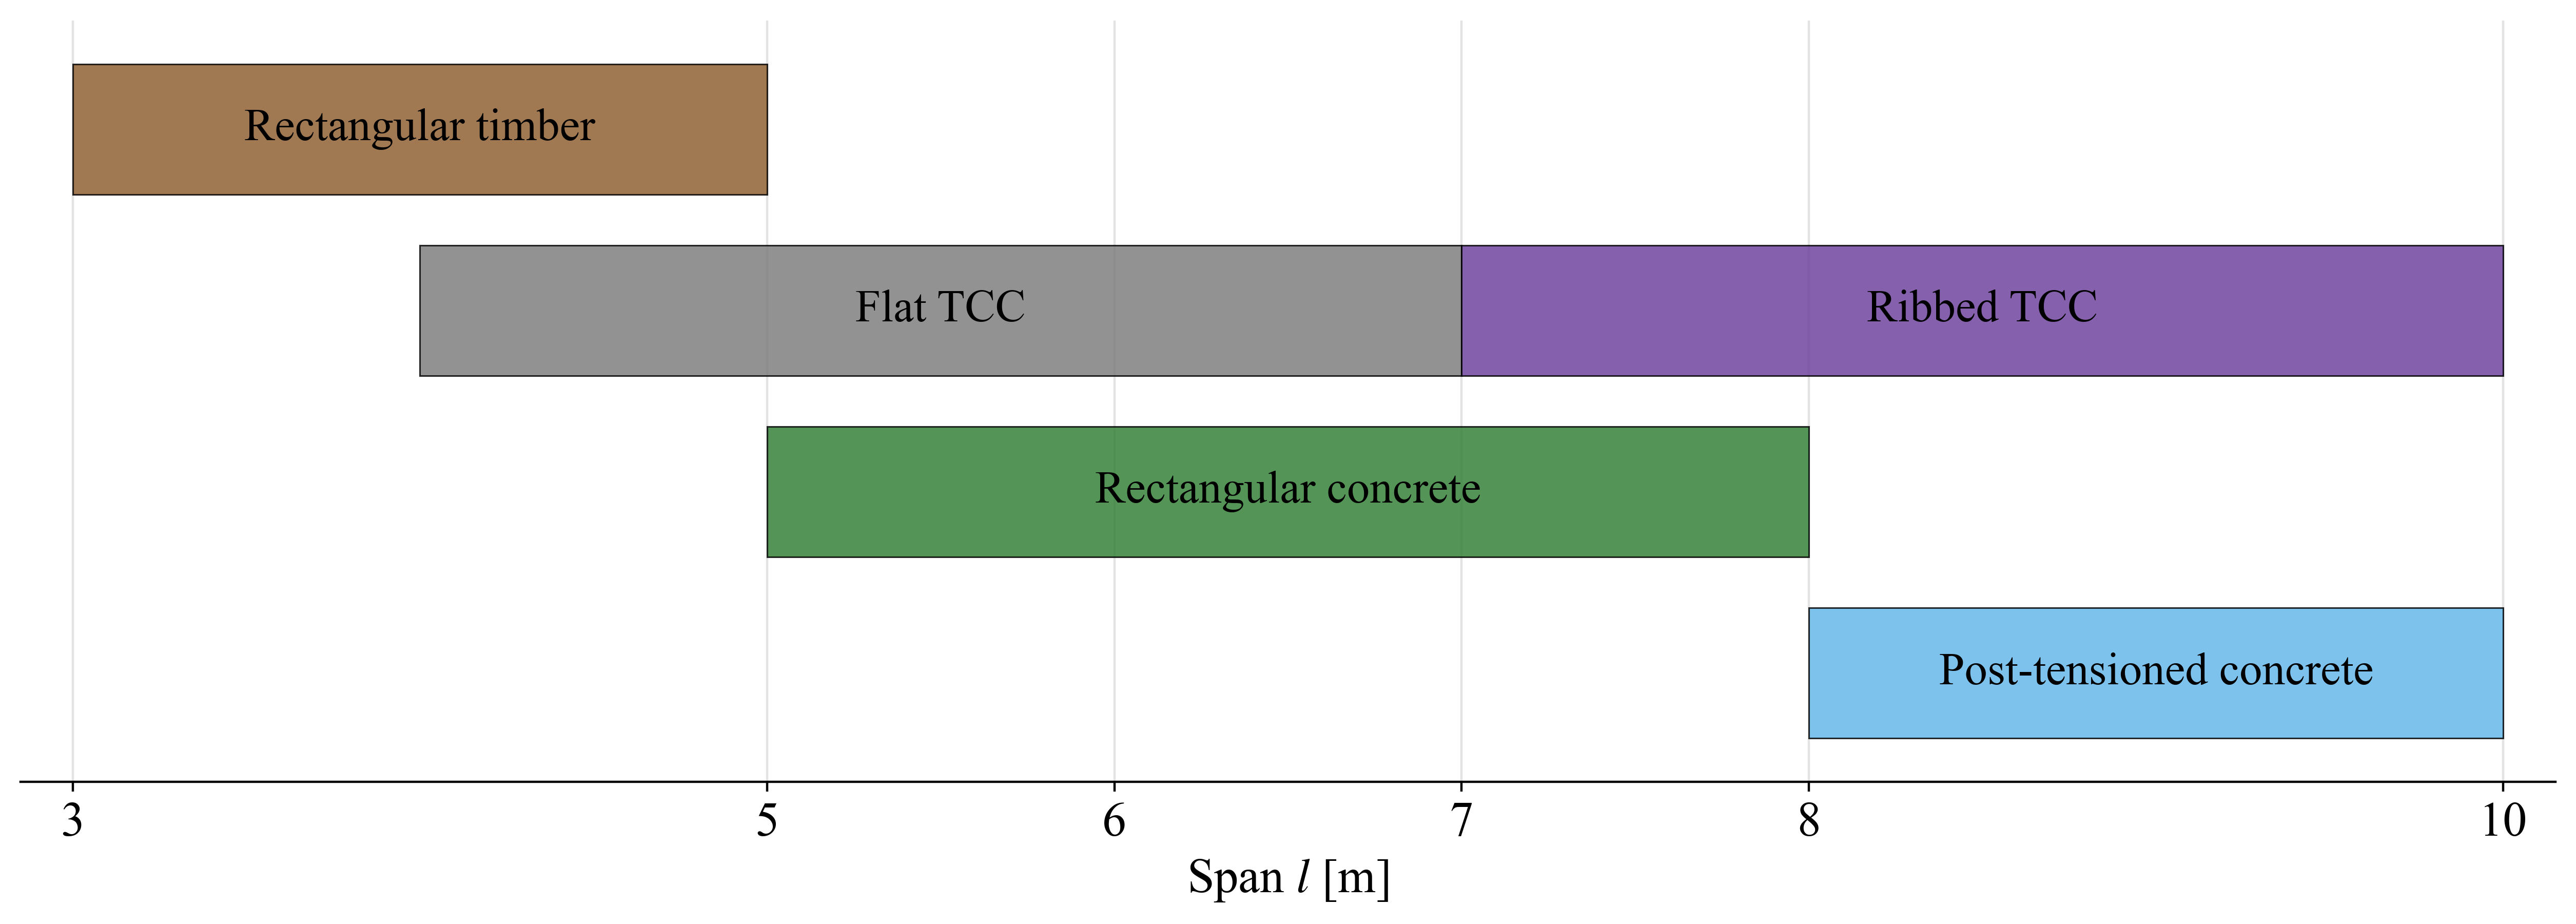
\includegraphics[width=1\textwidth]{IMAGES/final_application_ranges_residential.png}
    \caption{Proposed application ranges by span of compared systems for residential builings.}
    \label{fig:final_application_ranges_residential}
\end{figure}

The ribbed timber hollow-core system is lightweight but performs poorly regarding GWP and cost under the present assumptions. Its simplified fire verification and sensitivity to the selected insulation demonstrate the limitations of the configurator for highly specialised systems. More detailed fire checks and manufacturer-specific product data would be required for a conclusive assessment. As a result, the timber hollow-core system is excluded from Figure \ref{fig:final_application_ranges_residential}.


\subsection{Slab systems for office builings}
The office comparison showed that no system performs best across all criteria and spans. Rectangular reinforced concrete is not recommended for the investigated span range. It is neither economically competitive nor functionally advantageous, as its material demand, construction height, and \(GWP_{struct}\) increase strongly with span.

Post-tensioned concrete provides the best overall balance. It combines low construction height with competitive \(GWP_{struct}\) and remains economically competitive at larger spans. The banded tendon layout is recommended across the full investigated span range. It benefits from tendons concentrated in the support strips and leaves the field regions largely free for further material-saving measures, such as formwork inlays. The distributed tendon layout is recommended only when a banded layout is not possible and only up to approximately \(12\,\mathrm{m}\).

Ribbed concrete is recommended for spans from approximately \(10\) to \(16\,\mathrm{m}\), where its reduced material demand leads to favourable environmental and economic performance. However, it requires a larger construction depth and may therefore be excluded when floor height is a governing constraint.
\begin{figure}[H]
    \centering
    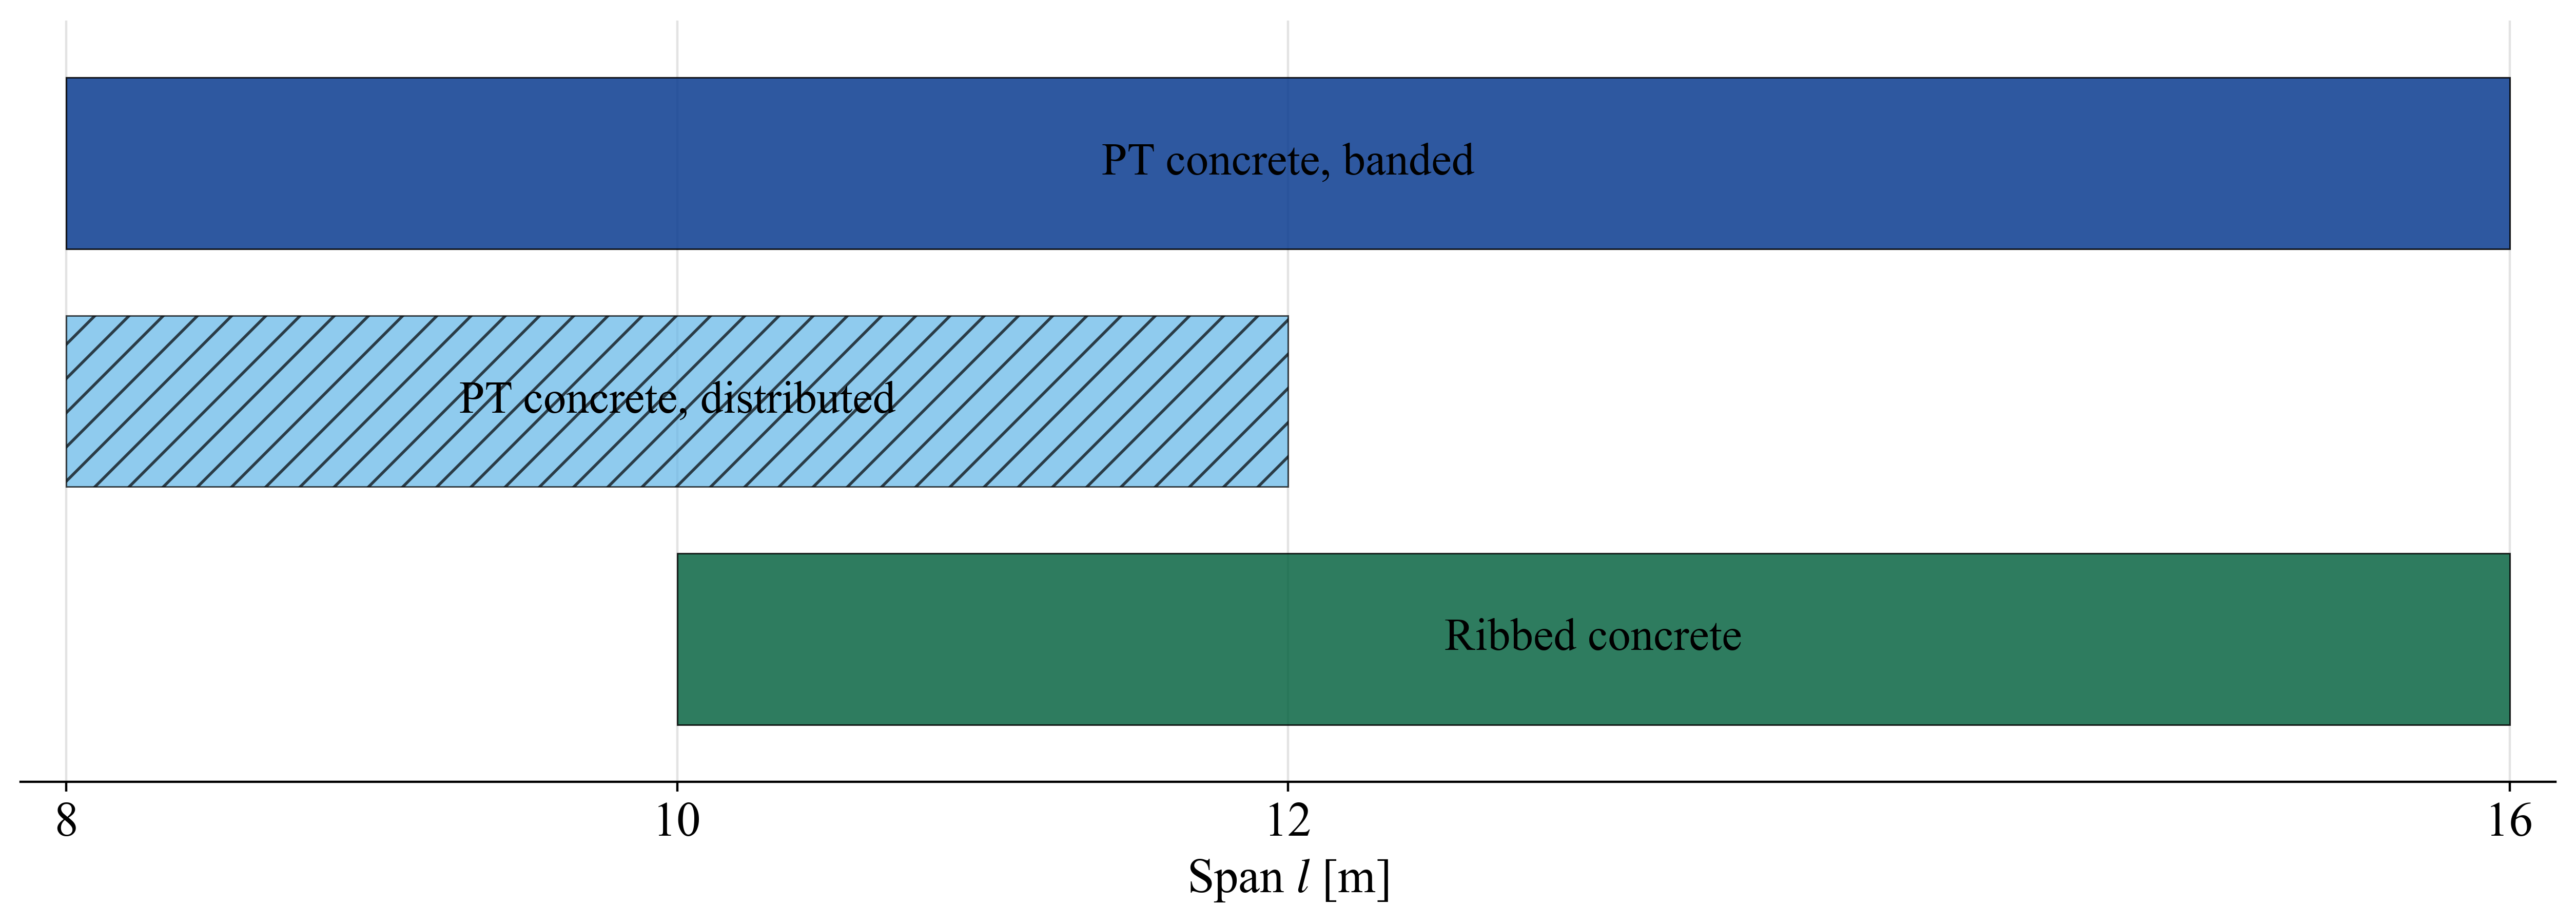
\includegraphics[width=1\textwidth]{IMAGES/final_application_ranges_office.png}
    \caption{Proposed application ranges by span of compared systems for office buildings.}
    \label{fig:final_application_ranges_office}
\end{figure}






